\documentclass[colorback,accentcolor=tud1c,11pt]{tudreport}
\usepackage[english]{babel}
\usepackage[utf8x]{inputenc}
%\usepackage[T1]{fontenc}

%\usepackage[stable]{footmisc}
%\usepackage[ngerman,pdfview=FitH,pdfstartview=FitV]{hyperref}

\usepackage{booktabs}
%\usepackage{multirow}
%\usepackage{longtable}
\usepackage{listings}
\usepackage{graphicx}
\usepackage{subfigure} 	
\usepackage{float}
\usepackage{amsmath}

\newcommand\todo[1]{\textcolor{red}{#1}}
\newcommand\code[1]{\texttt{#1}}
%\usepackage{floatflt}

\graphicspath{{./img/}}

%\newlength{\longtablewidth}
%\setlength{\longtablewidth}{0.675\linewidth}

\title{Mini-task report: Espresso Logic Minimization}
\subtitle{Mitja Stachowiak, Ludwig Meysel}

\begin{document}
  \maketitle

  \chapter{Introduction}

  The task was to implement a simple verino of the logic minimization algorithm ESPRESSO. Given are non-hierarchical BLIF files which can define one or more output variables. There must be found a efficient encoding for a positional cube notation. After running ESPRESSO on the boolean function the minimized function should be written again as a BILF file.

  \chapter{BLIF Parser}

  For the Minitasks a BLIF parser for finite state machines is given. A short analysis of the given parser makes it easy to implement the own parser for the simpler BLIF data. There is no need to consider any status information, but just the input combinations and the outputs for them. Fig.~\ref{fig:egblif1} shows a simple example of a boolean function defined in BLIF. The function consists only of an ON-set, the DC-set is neglegted at this point.

  \begin{figure}
	  \centering
	  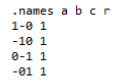
\includegraphics{img-blif}
	  \caption{Example for a BLIF defined boolean function}
	  \label{fig:egblif1}
  \end{figure}

  Starting with a filename given to a parser-method the parser creates a \code{Model} object which then contains a list of \code{BinFunction}s with their named inputs and outputs. Fig.~\ref{fig:egblif1} shows just one boolean function, but a BLIF file could contain multiple of them. It can even refer to other BLIF files. Therefore the \code{Model}-object contains a list of \code{BinFunction}s.
  \\
  The parser reads the input variables and encodes them in positional cube notation in Java's \code{long} primitive. In the positional cube notation each boolean varible is encoded with two bits. A \code{long} has 64 bits and can therefore handle 32 boolean variables in positional cube noation, within one long-variable. To be able to handle more than 32 boolean variables, a \code{Cube}-object handles a \code{long}-Array which makes it theoretically possible to handle arbitrary numbers of boolean variables. Actually there are other (physical) limits for the number of boolean variables, which at least are made up with the size of the internal memory.
  \\
  Espresso must be able to handle nearly each posible input combination in one \code{BinFunction}. When there are 32 input varbiables for one function, there are nearly $2^{32}$ possible input combinations, each taking one \code{long}-value. Therefore the required memory for a 32-input-\code{BinFunction} would be up to $2^{32} \times 4 Byte \sim 16 GB$! This space requirement doubles which each more input variable. It is therefore a discussion point whether it makes sense to implement a cube with a \code{long}-array or just set a limit in our implementation by using just one \code{long}. On the one hand it is nice to have an algorithm which is not limited by its implementation. On the other hand using just one \code{long}-value avoids the necessity of calculating the array-offset when checking one specific variable, which could save time because it avoids many divisions. In our implementation we decided for the first approach, using the \code{long}-array.
  

  \chapter{Implementation of Espresso}
  Espresso runs mainly in two phases \cite{micheli2003synthesis}:
  \begin{itemize}
  	\item{compute the complement}
	\begin{item}
		Iterate until cost function not further shrinks
		\begin{itemize}
			\item{expand}
			\item{remove irredundant cubes}
			\item{reduce}
		\end{itemize}
	\end{item}
  \end{itemize}

  \section{Computation of the complement}
  We decided to spare the computation of the function complement - there are more or less easy-to-implement approaches which handle different problems coming up with the computation. One of the main challenges of the complement computation is as already mentioned before: Memory. Having a 32-input-\code{BinFunction} would at least now lead to a memory-problem if the complement cannot be computed directly optimized.
  \par
  A straight-forward approach would be to iterate over each combination of the function and remove all those which are already included in the ON-set or the DC-set. But using a 32-input-function again would result in a huge amount of implicants, which require a lot of memory. Additionally, checking the expanded cubes against the non-optimized OFF-set results in very much iterations. So it is obvious that calculating the complement does only make sense when getting a more or less simplified result. There exist approaches for that, but this task was more about implementing espresso therefore we decided to spare the computation of the OFF-set and used the technique from PRESTO. This is instead of computing OFF-set and checking the expanded cubes against it, just checking if the expanded cubes aginst the ON- and DC-set.
  \par
  The drawback of this approach is that any expanded cube must be checked against the full ON- and DC-set, to detect coverage. Having a relatively small function, say 10 input variables ($2^{10}=1024$ possible combinations) with 100 cubes forming the ON- and DC-set, there are 924 implicants remaining in the OFF-set. That means the most expansions will collide with the OFF-set. That does also mean that checking against the OFF-set would not require to iterate over the full OFF-set, because when one collision is found, the iteration can be stopped. Furthermore when having a minimized OFF-set, it is pretty likely that it has only few cubes with many dont-cares.
  \par
  According to the lecture, it is already known, that ESPRESSO in general would run faster with the initial complement computation instead of using the PRESTO approach. We decided for the PRESTO approach, however, to focus on the ESPRESSO implementation itselft, but not on the complement computation.

 \section{Expansion}

  \bibliographystyle{plain}
  \bibliography{references}
\end{document}

